\section{Results}

Given sets $D$ and $E$ such that
$f : D \rightarrow E$ for $f$ a Boolean function,
we construct matrices corresponding to the constraints
in \cref{Eq:boyd_obj}.
Our implementation uses Python3 and the NumPy library \cite{numpy}.
We build $A_i$ for $i \in [|F|]$ to enforce the condition
outlined in \cref{Eq:off-diag} and set $b_i=1$.
We build $\Ap_i$ for $i \in [|D|]$ to enforce
that $z$ is the maximum $c_i$ and set $\bp_i = 0$.
Finally, we build $C$ to select $z$ from $\Xb$. To solve the SDP with our constraints,
we implemented Wen et al.'s ADM algorithm.



So far we have illustrated the SDP and its solution
through the example of the OR function.
Recall that OR takes as input $n$ bit strings
and returns 0 if there are no 1s in the input
and 1 otherwise.
We extend our analysis of OR by illustrating
an application of our SDP solver. Figures are made using a variety of functions from both data.table and tidyverse R packages \cite{tidyverse, data.table}.

\begin{figure}[ht]
\centering
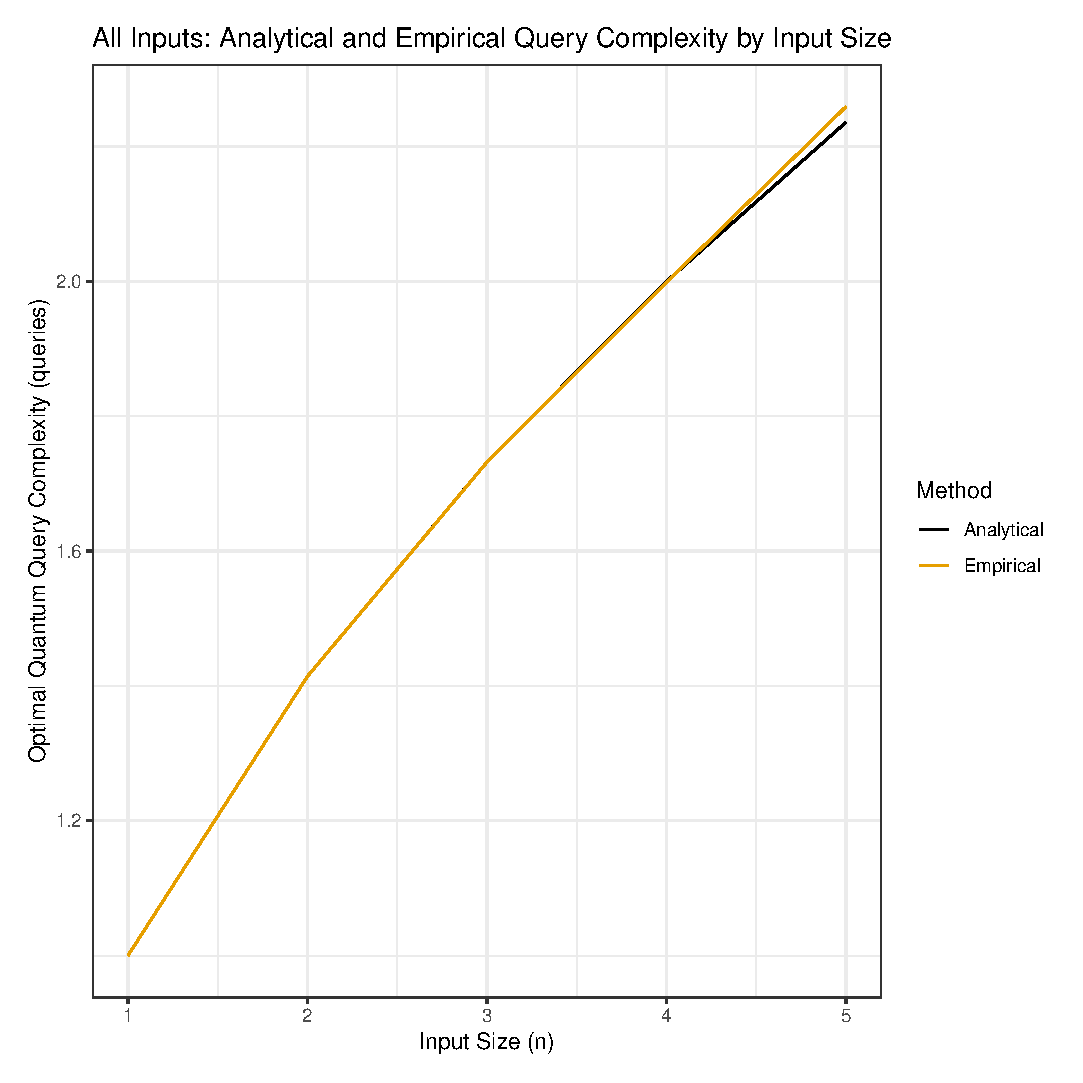
\includegraphics[scale=.5]{figure_all_or_complexity}
\caption{The proven analytical optimal query complexity
and calculated empirical optimal query complexity by 
size of input bit string.}
\end{figure}

\begin{figure}[ht]
\centering
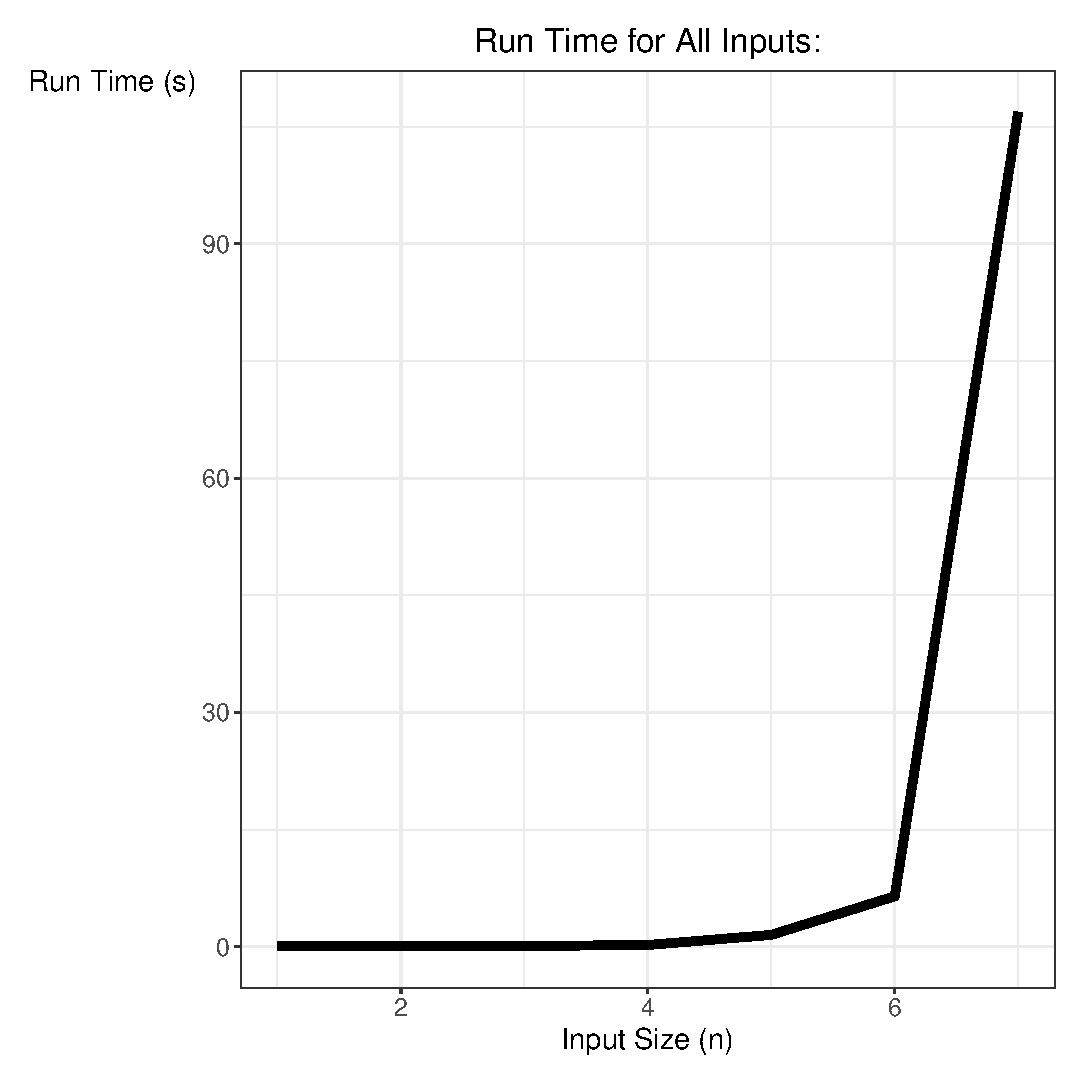
\includegraphics[scale=.4]{figure_all_or_time}
\caption{Run time of SDP solver by size of input strings.}
\end{figure}

\subsection{OR Function: Worst-case Boolean Inputs}\label{sec:speed}

Our algorithm's performance is visualized above. We see that run time grows exponentially with respect to input size as expected, given the exponential increase in the cardinality of the set $D$ of all inputs of length $n$. We also see that our algorithm is accurately calculating the optimal quantum query complexity of the OR function. 

Using the known results of the quantum query
complexity of the OR function along with our
algorithm's performance in regard to the known
optimal values, we believe that our algorithm is
correct. Proof's of the algorithm's mathematical
correctness can be found in Wen et. al. Proof of the
algorithm's is shown through these results as well as
review of our code posted on GitHub. Knowing that our
algorithm is correct, we can then proceed to improve
it in several ways. 

First, we can attempt to improve run time while
maintaining the correctness of the algorithm. Later,
we might be able to alter the algorithm
mathematically to take advantage of the structure
given in SDP's formed from quantum algorithms. 
It has also been claimed that the dual of this semidefinite
programming problem yields the quantum algorithm with minimal query complexity.
However, this optimal solution to the dual may not be easily 
interpreted as an algorithm as there could be many optimal, feasible solutions. 
Semidefinite programming problems also don't guarantee the tightness of the dual,
as is the case in linear programming. 
These problems all pose potential areas of future expansion.

\subsection{OR Function: All Boolean Inputs}

A simple approach to speeding up the runtime of our
algorithm is to simply decrease the number of input
strings considered for a given input size $n$. It's
important that we still obtain a good approximation
of the correct answer, so we need to ensure that the
inputs we do analyze will lead to the correct result.
Because the bounds of our algorithm are adversarial,
meaning that they are worst-case bounds, we can opt
to only use the worst-case inputs.

Again returning to our OR example, the hardest inputs are either entirely zeros, or contain only a single 1. Using these inputs, we can then run our algorithm to compare both runtime and precision of results.

\begin{figure}[ht]
\centering
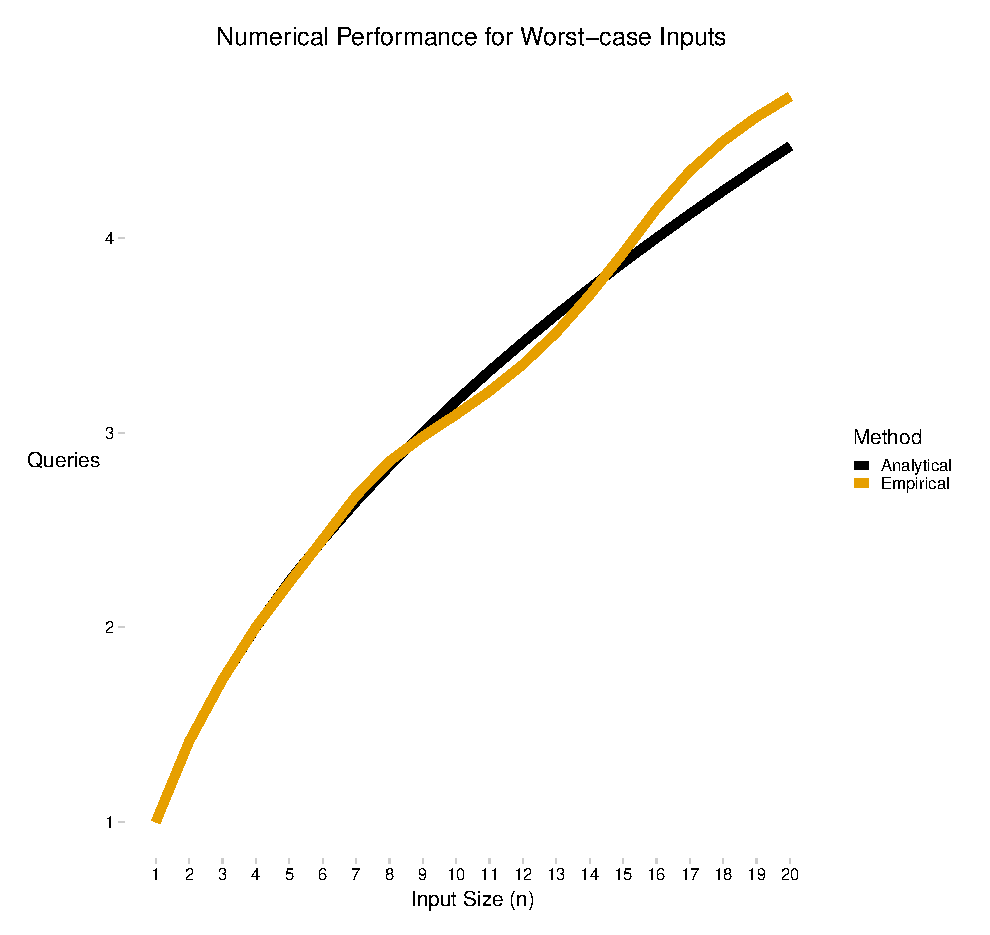
\includegraphics[scale=.5]{figure_worst_or_complexity}
\caption{The proven analytical optimal query complexity
and calculated empirical optimal query complexity by 
size of input bit string.}
\end{figure}

\begin{figure}[ht]
\centering
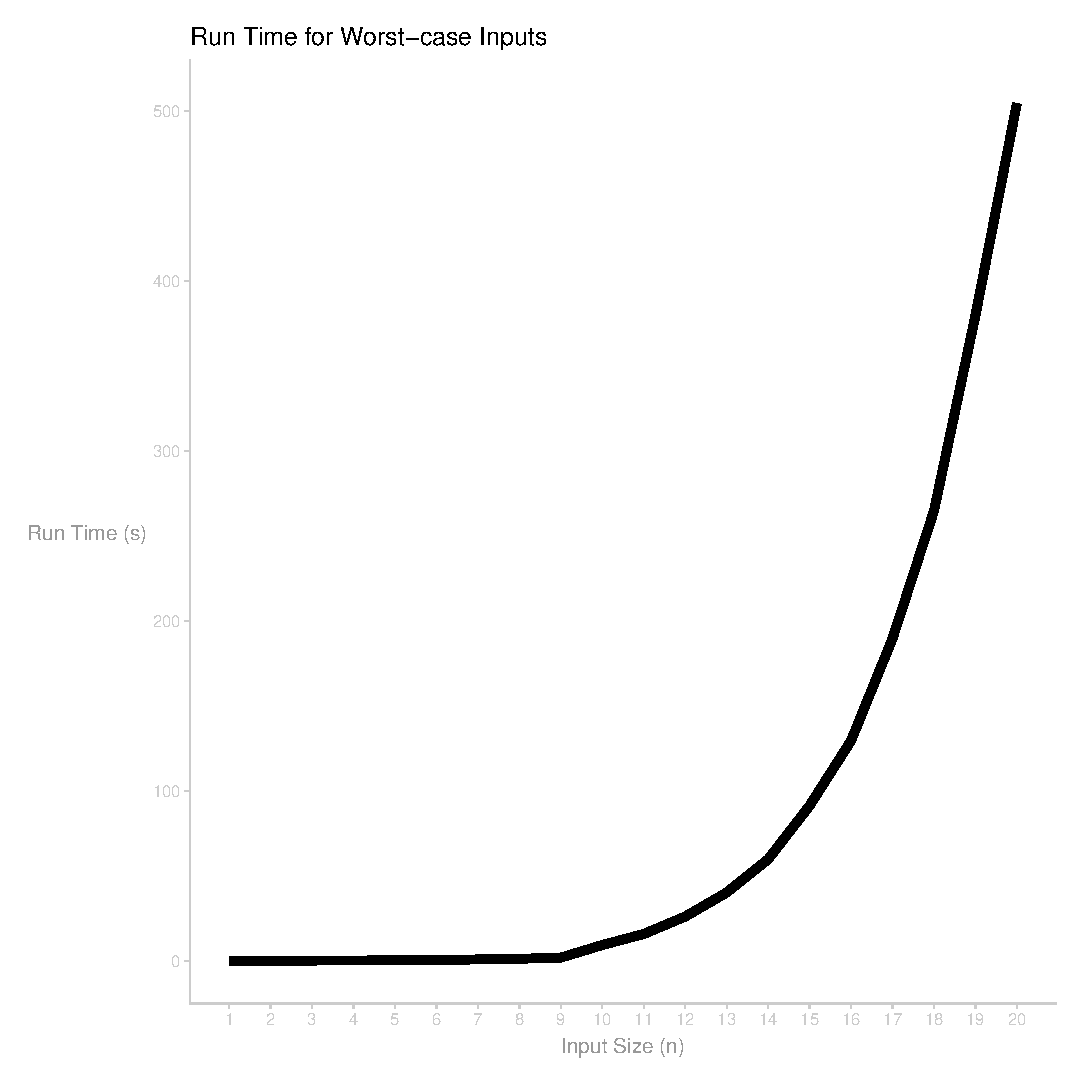
\includegraphics[scale=.4]{figure_worst_or_time}
\caption{Run time of SDP solver by size of input strings.}
\end{figure}

The run time is drastically improved over the all-case scenario. This result is not only show via the y-axis of the graphs, but also in the x-axis because the speed up was so significant that we were able to solve for many more input sizes than in the all-case scenario. 
Looking at the optimal query complexities returned, we observe that we are still obtaining good approximations of the true value. We believe that more iterations could drastically improve the performance of the algorithm as well as improved stopping conditions. Instead of simply stopping after some number of iterations (in this case 100), we could look to see if the improvements to the objective function are negligible and conclude that the algorithm has converged.
